%% Font size %%
\documentclass[11pt]{article}

%% Load the custom package
\usepackage{Mathdoc}

%% Numéro de séquence %% Titre de la séquence %%
\renewcommand{\centerhead}{Chap. 3 : Identitifer les angles particuliers}

%% Spacing commands %%
\renewcommand{\baselinestretch}{1}
\setlength{\parindent}{0pt}

\begin{document}

\section{Identifier les angles particuliers}


\begin{exercice}[1]
\textbf{Les angles marqués sont-ils alternes-internes, correspondants ou ni l'un, ni l'autre ?}
\begin{multicols}{3}
\begin{enumerate}
	\item \begin{minipage}[t]{\linewidth} 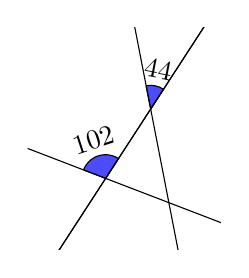
\begin{tikzpicture}[baseline,scale = 0.3]

    \tikzset{
      point/.style={
        thick,
        draw,
        cross out,
        inner sep=0pt,
        minimum width=5pt,
        minimum height=5pt,
      },
    }
    \clip (-4.390019349521659,-4.69335283972712) rectangle (3.78572476438357,4.702887402261128);
    	\draw  [color={black},preaction={fill,color = {blue},opacity = 0.7}] (0.626149557145996,2.2396330353657996) -- (0.8169585525225405,1.2580058519181354) -- (1.3615975875375679,2.0966764198635595) arc (56.72:100.72:1) ;
	\draw[color={black}] (-8.723491216304707,50.33936502430133)--(10.548217316726333,-48.804980503912724);
	\draw[color={black}] (-26.414993198228814,-40.67552254535305)--(28.59354933828892,44.030204817134745);
	\draw  [color={black},preaction={fill,color = {blue},opacity = 0.7}] (-2.0228584965272556,-1.3189731863455467) -- (-1.0892780700300544,-1.6773411358908479) -- (-0.5446390350150268,-0.8386705679454244) arc (56.72:158.72:1) ;
	\draw[color={black}] (-47.76829939489014,16.241056341374165)--(46.523323681327234,-19.954106562701163);
	\draw[color={black}] (-28.321229820781415,-43.610869533162045)--(26.687312715736333,41.094857829325775);
	\draw [color={black}] (1.14,2.93) node[anchor = center,scale=1, rotate = -10.995039999999989] {\ang{44}};
	\draw [color={black}] (-1.61,-0.06) node[anchor = center,scale=1, rotate = -341.99936] {\ang{102}};

\end{tikzpicture}\\ \end{minipage}
	\item \begin{minipage}[t]{\linewidth} 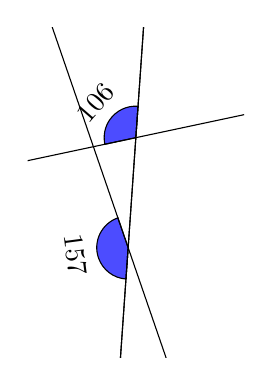
\begin{tikzpicture}[baseline,scale = 0.4]

    \tikzset{
      point/.style={
        thick,
        draw,
        cross out,
        inner sep=0pt,
        minimum width=5pt,
        minimum height=5pt,
      },
    }
    \clip (-3.329808091585229,-5.487820251299121) rectangle (3.539077512817605,4.989038226169209);
    	\draw  [color={black},preaction={fill,color = {blue},opacity = 0.7}] (-0.8735128901176171,1.2884343845719772) -- (0.1046347106161884,1.4963460753897364) -- (0.17439118436031364,2.4939101256495606) arc (85.69:191.69:1) ;
	\draw[color={black}] (-48.802745326074096,-8.899238465498234)--(49.99016234804028,12.099842307095466);
	\draw[color={black}] (-3.3831889765900853,-48.381856437601485)--(3.662214871566587,52.372112638640786);
	\draw  [color={black},preaction={fill,color = {blue},opacity = 0.7}] (-0.20926942123237727,-2.992692150779473) -- (-0.1395129474882513,-1.9951281005196484) -- (-0.4650811019454078,-1.0496095249203314) arc (109.17:266.17:1) ;
	\draw[color={black}] (-16.41792067034609,45.280800679446195)--(16.464462929826745,-50.21657545608481);
	\draw[color={black}] (-3.627336634694524,-51.87333061351086)--(3.4180672134621473,48.88063846273138);
	\draw [color={black}] (-1.18,2.61) node[anchor = center,scale=1, rotate = -311.0002] {\ang{106}};
	\draw [color={black}] (-1.82,-2.22) node[anchor = center,scale=1, rotate = -82.50011] {\ang{157}};

\end{tikzpicture}\\ \end{minipage}
	\item \begin{minipage}[t]{\linewidth} 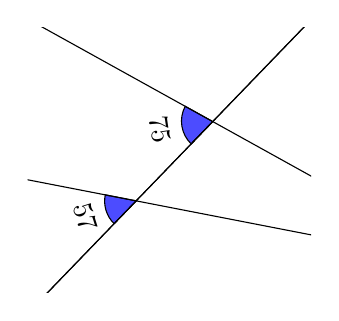
\begin{tikzpicture}[baseline,scale = 0.4]

    \tikzset{
      point/.style={
        thick,
        draw,
        cross out,
        inner sep=0pt,
        minimum width=5pt,
        minimum height=5pt,
      },
    }
    \clip (-4.486869106031488,-4.000328516779962) rectangle (4.5131758623361815,4.4200065683925605);
    	\draw  [color={black},preaction={fill,color = {blue},opacity = 0.7}] (0.6946583704589984,0.7193398003386509) -- (1.3893167409179954,1.4386796006773026) -- (0.5146970337785991,1.9234892209236392) arc (151.86:226.86:1) ;
	\draw[color={black}] (-42.34166861605179,25.679160612994153)--(45.99492180502718,-23.286611031885883);
	\draw[color={black}] (-33.343601782031854,-34.52831041625525)--(36.816893634326846,38.12500941794851);
	\draw  [color={black},preaction={fill,color = {blue},opacity = 0.7}] (-1.7366459261474938,-1.798349500846627) -- (-1.0419875556884963,-1.0790097005079757) -- (-2.0236147391361605,-0.8882007051314311) arc (168.54:225.54:1) ;
	\draw[color={black}] (-50.123346728071695,8.461440068319265)--(49.02099880014237,-10.810268464711761);
	\draw[color={black}] (-35.77490607863836,-37.04599971744053)--(34.38558933772037,35.60732011676323);
	\draw [color={black}] (-0.29,1.19) node[anchor = center,scale=1, rotate = -81.50019] {\ang{75}};
	\draw [color={black}] (-2.66,-1.59) node[anchor = center,scale=1, rotate = -72.49962] {\ang{57}};

\end{tikzpicture}\\ \end{minipage}
	\item \begin{minipage}[t]{\linewidth} 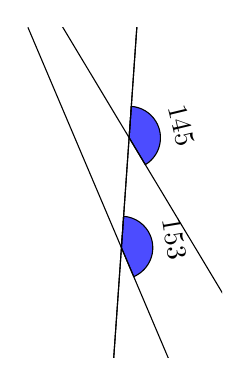
\begin{tikzpicture}[baseline,scale = 0.4]

    \tikzset{
      point/.style={
        thick,
        draw,
        cross out,
        inner sep=0pt,
        minimum width=5pt,
        minimum height=5pt,
      },
    }
    \clip (-3.081320233229482,-4.989038226169209) rectangle (3.0925418121643005,5.487820251299121);
    	\draw  [color={black},preaction={fill,color = {blue},opacity = 0.7}] (0.20926942123237668,2.992692150779472) -- (0.1395129474882511,1.9951281005196482) -- (0.6545510223983052,1.1379607998175363) arc (-58.68:86.32:1) ;
	\draw[color={black}] (-25.612390798014463,44.85349313562526)--(26.406454767901018,-41.72040423528807);
	\draw[color={black}] (-3.348310739718021,-47.88307441247155)--(3.6970931084386485,52.87089466377067);
	\draw  [color={black},preaction={fill,color = {blue},opacity = 0.7}] (-0.034878236872062596,-0.4987820251299113) -- (-0.10463471061618815,-1.496346075389736) -- (0.2860964178730856,-2.4168509288421767) arc (-66.73:86.27:1) ;
	\draw[color={black}] (-19.641191135079886,44.52889659723229)--(19.822652842336783,-48.44209360146421);
	\draw[color={black}] (-3.5924583978224613,-51.37454858838095)--(3.45294545033421,49.379420487861296);
	\draw [color={black}] (1.79,2.39) node[anchor = center,scale=1, rotate = -76.50006] {\ang{145}};
	\draw [color={black}] (1.57,-1.22) node[anchor = center,scale=1, rotate = -80.50002] {\ang{153}};

\end{tikzpicture}\\ \end{minipage}
	\item \begin{minipage}[t]{\linewidth} 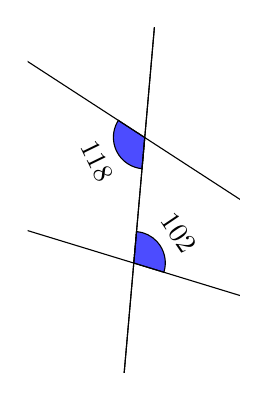
\begin{tikzpicture}[baseline,scale = 0.4]

    \tikzset{
      point/.style={
        thick,
        draw,
        cross out,
        inner sep=0pt,
        minimum width=5pt,
        minimum height=5pt,
      },
    }
    \clip (-3.543225753384422,-5.480973490458728) rectangle (3.1946027823937895,5.480973490458728);
    	\draw  [color={black},preaction={fill,color = {blue},opacity = 0.7}] (0.08715574274765758,0.9961946980917454) -- (0.17431148549531622,1.9923893961834909) -- (-0.6643590824501077,2.537028431198518) arc (147.48:265.48:1) ;
	\draw[color={black}] (-41.75921691177589,29.22434114693484)--(42.94651045071194,-25.784201389582886);
	\draw[color={black}] (-4.183475651887591,-47.8173455084038)--(4.619254365625881,52.79831899886253);
	\draw  [color={black},preaction={fill,color = {blue},opacity = 0.7}] (-0.08715574274765814,-0.9961946980917457) -- (-0.17431148549531658,-1.992389396183491) -- (0.7819932704677189,-2.284761100906228) arc (-17.25:84.75:1) ;
	\draw[color={black}] (-47.98954928364709,12.626195839953347)--(48.597231068619486,-16.903346337043065);
	\draw[color={black}] (-4.532098622878223,-51.80212430077077)--(4.270631394635249,48.81354020649553);
	\draw [color={black}] (-1.35,1.25) node[anchor = center,scale=1, rotate = -64.00014] {\ang{118}};
	\draw [color={black}] (1.24,-1.04) node[anchor = center,scale=1, rotate = -55.999719999999996] {\ang{102}};

\end{tikzpicture}\\ \end{minipage}
	\item \begin{minipage}[t]{\linewidth} 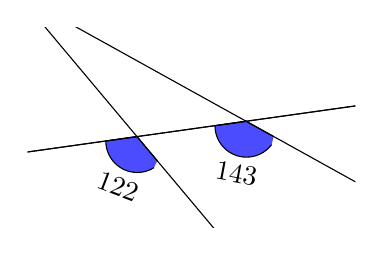
\begin{tikzpicture}[baseline,scale = 0.4]

    \tikzset{
      point/.style={
        thick,
        draw,
        cross out,
        inner sep=0pt,
        minimum width=5pt,
        minimum height=5pt,
      },
    }
    \clip (-4.956206309337067,-3.0958463764853414) rectangle (5.451340343707852,3.249879544778853);
    	\draw  [color={black},preaction={fill,color = {blue},opacity = 0.7}] (2.8551558446225362,-0.20646341832620585) -- (1.9805361374831405,0.27834620192013104) -- (0.9902680687415701,0.13917310096006552) arc (-180:-37:1) ;
	\draw[color={black}] (-41.75044921948663,24.518827214236982)--(46.58614120159231,-24.446944430643057);
	\draw[color={black}] (-47.53286729959539,-6.680308846083142)--(52.48420764330324,7.37617435088347);
	\draw  [color={black},preaction={fill,color = {blue},opacity = 0.7}] (-0.842614493425816,-0.9748040945590766) -- (-1.4854021031123552,-0.20875965144009823) -- (-2.475670171853926,-0.34793275240016364) arc (-180:-58:1) ;
	\draw[color={black}] (-33.62478258743933,38.09346250450881)--(31.296765990901154,-39.27702625050798);
	\draw[color={black}] (-50.99880554019087,-7.16741469944337)--(49.01826940270773,6.889068497523239);
	\draw [color={black}] (1.67,-1.39) node[anchor = center,scale=1, rotate = -10.49892] {\ang{143}};
	\draw [color={black}] (-2.09,-1.8) node[anchor = center,scale=1, rotate = -20.99966] {\ang{122}};

\end{tikzpicture}\\ \end{minipage}
	\item \begin{minipage}[t]{\linewidth} 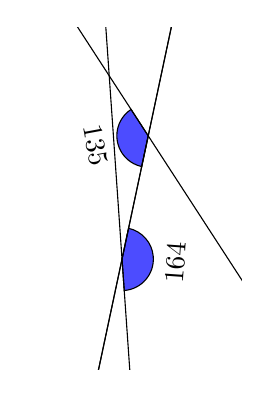
\begin{tikzpicture}[baseline,scale = 0.4]

    \tikzset{
      point/.style={
        thick,
        draw,
        cross out,
        inner sep=0pt,
        minimum width=5pt,
        minimum height=5pt,
      },
    }
    \clip (-3.4116822670772207,-5.448987352247084) rectangle (3.387356724494242,5.390738003669028);
    	\draw  [color={black},preaction={fill,color = {blue},opacity = 0.7}] (0.20791169081775973,0.9781476007338062) -- (0.4158233816355189,1.9562952014676114) -- (-0.12881565337950807,2.794965769413035) arc (123.28:258.28:1) ;
	\draw[color={black}] (-26.816128369115834,43.8898235987388)--(28.1924141674019,-40.815903763749);
	\draw[color={black}] (-9.979761159252451,-46.95108483522266)--(11.01931961334125,51.84182283889169);
	\draw  [color={black},preaction={fill,color = {blue},opacity = 0.7}] (-0.20791169081775984,-0.9781476007338058) -- (-0.4158233816355195,-1.9562952014676112) -- (-0.3460669078913941,-2.9538592517274354) arc (-85.69:78.31:1) ;
	\draw[color={black}] (-3.903647068841793,47.9219073115236)--(3.1417567793148793,-52.832061764718645);
	\draw[color={black}] (-10.811407922523491,-50.86367523815789)--(10.187672850070213,47.92923243595647);
	\draw [color={black}] (-1.26,1.65) node[anchor = center,scale=1, rotate = -79.4997] {\ang{135}};
	\draw [color={black}] (1.28,-2.07) node[anchor = center,scale=1, rotate = 85.99994] {\ang{164}};

\end{tikzpicture}\\ \end{minipage}
	\item \begin{minipage}[t]{\linewidth} 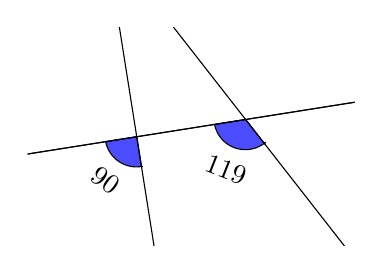
\begin{tikzpicture}[baseline,scale = 0.4]

    \tikzset{
      point/.style={
        thick,
        draw,
        cross out,
        inner sep=0pt,
        minimum width=5pt,
        minimum height=5pt,
      },
    }
    \clip (-4.94459753267812,-3.6977167193457596) rectangle (5.438441702975689,3.228413324225068);
    	\draw  [color={black},preaction={fill,color = {blue},opacity = 0.7}] (2.5910381565159337,-0.4751418235262608) -- (1.9753766811902758,0.3128689300804615) -- (0.9876883405951378,0.15643446504023095) arc (-168.54:-49.53999999999999:1) ;
	\draw[color={black}] (-28.807697085092634,39.71340661041656)--(33.374111922798846,-39.87567950386236);
	\draw[color={black}] (-47.40904034856661,-7.508854321931083)--(52.3474820515423,8.291026647132238);
	\draw  [color={black},preaction={fill,color = {blue},opacity = 0.7}] (-1.3250980458524761,-1.2223400381554839) -- (-1.4815325108927069,-0.234651697560346) -- (-2.4692208514878446,-0.3910861626005768) arc (-168.54:-78.53999999999999:1) ;
	\draw[color={black}] (-9.303255762904255,49.149765332196544)--(6.496625206159072,-50.606757067912376);
	\draw[color={black}] (-50.865949540649595,-8.05637494957189)--(48.89057285945932,7.743506019491428);
	\draw [color={black}] (1.35,-1.27) node[anchor = center,scale=1, rotate = -21.49967] {\ang{119}};
	\draw [color={black}] (-2.48,-1.61) node[anchor = center,scale=1, rotate = -36.00042] {\ang{90}};

\end{tikzpicture}\\ \end{minipage}
	\item \begin{minipage}[t]{\linewidth} 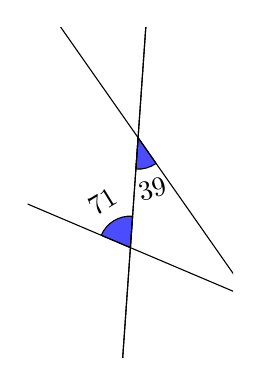
\begin{tikzpicture}[baseline,scale = 0.4]

    \tikzset{
      point/.style={
        thick,
        draw,
        cross out,
        inner sep=0pt,
        minimum width=5pt,
        minimum height=5pt,
      },
    }
    \clip (-3.3661492709735095,-4.989038226169209) rectangle (3.1568798497411326,5.487820251299121);
    	\draw  [color={black},preaction={fill,color = {blue},opacity = 0.7}] (0.7130893838392963,1.1759760562306565) -- (0.1395129474882508,1.9951281005196482) -- (0.06975647374412534,0.9975640502598244) arc (-93.77:-54.769999999999996:1) ;
	\draw[color={black}] (-28.539308870064048,42.95273031496924)--(29.391911201391594,-39.78162615821893);
	\draw[color={black}] (-3.348310739718021,-47.88307441247155)--(3.6970931084386485,52.87089466377067);
	\draw  [color={black},preaction={fill,color = {blue},opacity = 0.7}] (-1.0251395640686283,-1.1056149469004621) -- (-0.10463471061618831,-1.496346075389736) -- (-0.034878236872062915,-0.498782025129912) arc (85.69:156.69:1) ;
	\draw[color={black}] (-46.12987738323821,18.040210349073945)--(46.841112815458274,-21.42363362834269);
	\draw[color={black}] (-3.5924583978224613,-51.37454858838095)--(3.45294545033421,49.379420487861296);
	\draw [color={black}] (0.59,0.36) node[anchor = center,scale=1, rotate = 15.49952] {\ang{39}};
	\draw [color={black}] (-0.99,-0.05) node[anchor = center,scale=1, rotate = -328.49966] {\ang{71}};

\end{tikzpicture}\\ \end{minipage}
\end{enumerate}
\end{multicols}

\end{exercice}

\newpage

\section{Nommer les angles particuliers}

\begin{exercice}[1]
\begin{multicols}{3}
\begin{enumerate}
	\item \begin{minipage}[t]{\linewidth} Quel est l'angle alterne-interne à l'angle $\widehat{xDA}$ ?\\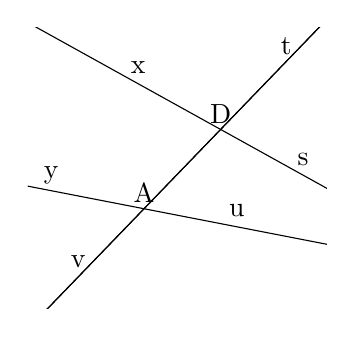
\begin{tikzpicture}[baseline,scale = 0.4]

    \tikzset{
      point/.style={
        thick,
        draw,
        cross out,
        inner sep=0pt,
        minimum width=5pt,
        minimum height=5pt,
      },
    }
    \clip (-4.736869106031488,-4.250328516779962) rectangle (4.7631758623361815,4.6700065683925605);
    	\draw[color={black}] (-42.34166861605179,25.679160612994153)--(45.99492180502718,-23.286611031885883);
	\draw[color={black}] (-33.343601782031854,-34.52831041625525)--(36.816893634326846,38.12500941794851);
	\draw[color={black}] (-50.123346728071695,8.461440068319265)--(49.02099880014237,-10.810268464711761);
	\draw[color={black}] (-35.77490607863836,-37.04599971744053)--(34.38558933772037,35.60732011676323);
	\draw [color={black}] (4.01,0.48) node[anchor = center,scale=1, rotate = 0] {s};
	\draw [color={black}] (-1.23,3.39) node[anchor = center,scale=1, rotate = 0] {x};
	\draw [color={black}] (3.47,4.1) node[anchor = center,scale=1, rotate = 0] {t};
	\draw [color={black}] (1.9,-1.15) node[anchor = center,scale=1, rotate = 0] {u};
	\draw [color={black}] (-3.99,-0.01) node[anchor = center,scale=1, rotate = 0] {y};
	\draw [color={black}] (-3.13,-2.74) node[anchor = center,scale=1, rotate = 0] {v};
	\draw [color={black}] (1.39,1.94) node[anchor = center,scale=1, rotate = 0] {D};
	\draw [color={black}] (-1.04,-0.58) node[anchor = center,scale=1, rotate = 0] {A};

\end{tikzpicture}\\ \end{minipage}
	\item \begin{minipage}[t]{\linewidth} Quel est l'angle alterne-interne à l'angle $\widehat{ADv}$ ?\\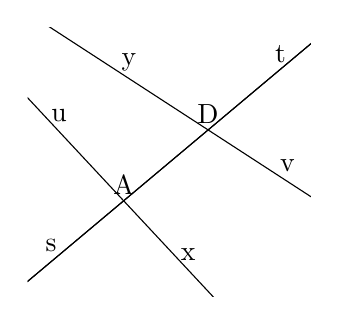
\begin{tikzpicture}[baseline,scale = 0.4]

    \tikzset{
      point/.style={
        thick,
        draw,
        cross out,
        inner sep=0pt,
        minimum width=5pt,
        minimum height=5pt,
      },
    }
    \clip (-4.197199994035402,-4.011010571846983) rectangle (4.798100590074228,4.532404376690253);
    	\draw[color={black}] (-40.40143951103323,28.51752697012443)--(44.30428785145457,-26.491015566393298);
	\draw[color={black}] (-36.770133269710925,-30.853805264953884)--(40.60035548530582,34.06774331338658);
	\draw[color={black}] (-35.24898466780339,35.603503666428715)--(33.632849698508956,-38.26322019710751);
	\draw[color={black}] (-39.45128882062737,-33.103561898856775)--(37.91919993438942,31.817986679483695);
	\draw [color={black}] (4.05,0.15) node[anchor = center,scale=1, rotate = 0] {v};
	\draw [color={black}] (-0.98,3.42) node[anchor = center,scale=1, rotate = 0] {y};
	\draw [color={black}] (3.83,3.71) node[anchor = center,scale=1, rotate = 0] {t};
	\draw [color={black}] (0.9,-2.66) node[anchor = center,scale=1, rotate = 0] {x};
	\draw [color={black}] (-3.2,1.73) node[anchor = center,scale=1, rotate = 0] {u};
	\draw [color={black}] (-3.45,-2.39) node[anchor = center,scale=1, rotate = 0] {s};
	\draw [color={black}] (1.53,1.79) node[anchor = center,scale=1, rotate = 0] {D};
	\draw [color={black}] (-1.15,-0.46) node[anchor = center,scale=1, rotate = 0] {A};

\end{tikzpicture}\\ \end{minipage}
	\item \begin{minipage}[t]{\linewidth} Quel est l'angle alterne-interne à l'angle $\widehat{BEy}$ ?\\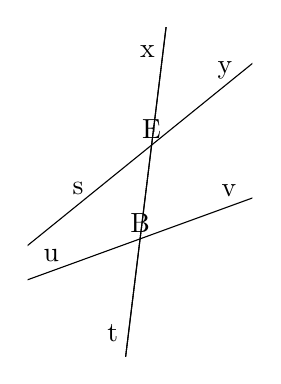
\begin{tikzpicture}[baseline,scale = 0.4]

    \tikzset{
      point/.style={
        thick,
        draw,
        cross out,
        inner sep=0pt,
        minimum width=5pt,
        minimum height=5pt,
      },
    }
    \clip (-3.751881877465446,-5.216457682385949) rectangle (3.3862738472500045,5.216457682385949);
    	\draw[color={black}] (-38.67449405774082,-29.977200325029884)--(39.81724804941324,33.584159171003684);
	\draw[color={black}] (-5.910663155149652,-48.13848835460412)--(6.3981405287702415,52.108672961169404);
	\draw[color={black}] (-47.16743505440314,-18.58982639374542)--(47.74151964497361,15.954208082147119);
	\draw[color={black}] (-6.276271185365095,-51.11612680952808)--(6.032532498554802,49.13103450624544);
	\draw [color={black}] (2.51,3.88) node[anchor = center,scale=1, rotate = 0] {y};
	\draw [color={black}] (-2.15,0.1) node[anchor = center,scale=1, rotate = 0] {s};
	\draw [color={black}] (0.05,4.47) node[anchor = center,scale=1, rotate = 0] {x};
	\draw [color={black}] (2.64,0.04) node[anchor = center,scale=1, rotate = 0] {v};
	\draw [color={black}] (-3,-2.01) node[anchor = center,scale=1, rotate = 0] {u};
	\draw [color={black}] (-1.05,-4.47) node[anchor = center,scale=1, rotate = 0] {t};
	\draw [color={black}] (0.18,1.99) node[anchor = center,scale=1, rotate = 0] {E};
	\draw [color={black}] (-0.18,-0.99) node[anchor = center,scale=1, rotate = 0] {B};

\end{tikzpicture}\\ \end{minipage}
	\item \begin{minipage}[t]{\linewidth} Quel est l'angle correspondant à l'angle $\widehat{uAt}$ ?\\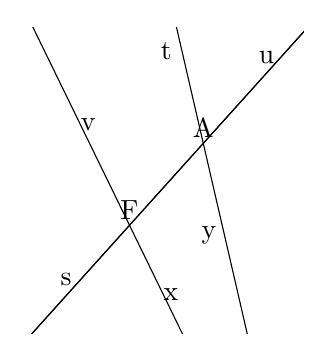
\begin{tikzpicture}[baseline,scale = 0.4]

    \tikzset{
      point/.style={
        thick,
        draw,
        cross out,
        inner sep=0pt,
        minimum width=5pt,
        minimum height=5pt,
      },
    }
    \clip (-4.571716929578387,-4.932671789852289) rectangle (4.199546898181071,4.787827432571796);
    	\draw[color={black}] (-10.243856807654957,49.83322047747786)--(12.476199681075396,-48.57815606583091);
	\draw[color={black}] (-32.45283440840463,-36.04252403565362)--(35.129356833840056,39.015103337563204);
	\draw[color={black}] (-23.256818552171588,43.45341266400355)--(21.01866727352523,-47.32478601221229);
	\draw[color={black}] (-34.79479153066063,-38.643530924824496)--(32.78739971158406,36.414096448392314);
	\draw [color={black}] (1.18,-1.81) node[anchor = center,scale=1, rotate = 0] {y};
	\draw [color={black}] (-0.17,4.04) node[anchor = center,scale=1, rotate = 0] {t};
	\draw [color={black}] (3.01,3.84) node[anchor = center,scale=1, rotate = 0] {u};
	\draw [color={black}] (-0.02,-3.68) node[anchor = center,scale=1, rotate = 0] {x};
	\draw [color={black}] (-2.65,1.71) node[anchor = center,scale=1, rotate = 0] {v};
	\draw [color={black}] (-3.35,-3.22) node[anchor = center,scale=1, rotate = 0] {s};
	\draw [color={black}] (1,1.61) node[anchor = center,scale=1, rotate = 0] {A};
	\draw [color={black}] (-1.34,-0.99) node[anchor = center,scale=1, rotate = 0] {F};

\end{tikzpicture}\\ \end{minipage}
	\item \begin{minipage}[t]{\linewidth} Quel est l'angle correspondant à l'angle $\widehat{yFu}$ ?\\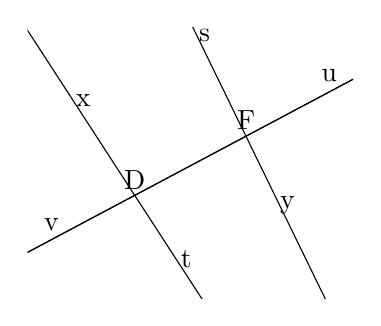
\begin{tikzpicture}[baseline,scale = 0.4]

    \tikzset{
      point/.style={
        thick,
        draw,
        cross out,
        inner sep=0pt,
        minimum width=5pt,
        minimum height=5pt,
      },
    }
    \clip (-5.164737964294635,-4.204954829408053) rectangle (5.164737964294635,4.385325264469283);
    	\draw[color={black}] (-20.152662153736017,45.878645440530136)--(24.122823671960802,-44.89955323568574);
	\draw[color={black}] (-42.381484457228495,-22.53463501372276)--(46.796222421523126,24.881992827652216);
	\draw[color={black}] (-28.997846936469212,40.99458527169941)--(26.010695600048535,-43.71114209078839);
	\draw[color={black}] (-45.9132748286642,-24.412521264866324)--(43.26443205008742,23.00410657650865);
	\draw [color={black}] (3.08,-1.26) node[anchor = center,scale=1, rotate = 0] {y};
	\draw [color={black}] (0.45,4.14) node[anchor = center,scale=1, rotate = 0] {s};
	\draw [color={black}] (4.41,2.85) node[anchor = center,scale=1, rotate = 0] {u};
	\draw [color={black}] (-0.13,-2.95) node[anchor = center,scale=1, rotate = 0] {t};
	\draw [color={black}] (-3.4,2.08) node[anchor = center,scale=1, rotate = 0] {x};
	\draw [color={black}] (-4.41,-1.85) node[anchor = center,scale=1, rotate = 0] {v};
	\draw [color={black}] (1.77,1.44) node[anchor = center,scale=1, rotate = 0] {F};
	\draw [color={black}] (-1.77,-0.44) node[anchor = center,scale=1, rotate = 0] {D};

\end{tikzpicture}\\ \end{minipage}
	\item \begin{minipage}[t]{\linewidth} Quel est l'angle alterne-interne à l'angle $\widehat{FCu}$ ?\\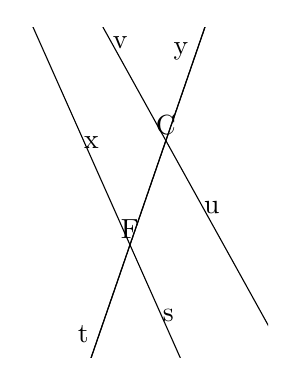
\begin{tikzpicture}[baseline,scale = 0.4]

    \tikzset{
      point/.style={
        thick,
        draw,
        cross out,
        inner sep=0pt,
        minimum width=5pt,
        minimum height=5pt,
      },
    }
    \clip (-3.7367342083748936,-5.004833590196926) rectangle (3.8946672956702804,5.4775928779965835);
    	\draw[color={black}] (-23.589344703402542,45.622022508168406)--(25.376426941477508,-42.71456791291054);
	\draw[color={black}] (-15.627271413943522,-45.38489162876719)--(17.255112186229304,50.11248450676377);
	\draw[color={black}] (-20.825184385475744,44.25899501873106)--(20.255216565180074,-48.009096203171616);
	\draw[color={black}] (-16.766759954543573,-48.694206643364815)--(16.11562364562926,46.80316949216618);
	\draw [color={black}] (2.11,-0.23) node[anchor = center,scale=1, rotate = 0] {u};
	\draw [color={black}] (-0.8,5.01) node[anchor = center,scale=1, rotate = 0] {v};
	\draw [color={black}] (1.13,4.73) node[anchor = center,scale=1, rotate = 0] {y};
	\draw [color={black}] (0.73,-3.66) node[anchor = center,scale=1, rotate = 0] {s};
	\draw [color={black}] (-1.71,1.82) node[anchor = center,scale=1, rotate = 0] {x};
	\draw [color={black}] (-1.97,-4.25) node[anchor = center,scale=1, rotate = 0] {t};
	\draw [color={black}] (0.65,2.39) node[anchor = center,scale=1, rotate = 0] {C};
	\draw [color={black}] (-0.49,-0.92) node[anchor = center,scale=1, rotate = 0] {F};

\end{tikzpicture}\\ \end{minipage}
	\item \begin{minipage}[t]{\linewidth} Quel est l'angle correspondant à l'angle $\widehat{uDx}$ ?\\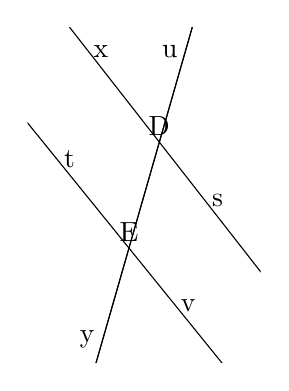
\begin{tikzpicture}[baseline,scale = 0.4]

    \tikzset{
      point/.style={
        thick,
        draw,
        cross out,
        inner sep=0pt,
        minimum width=5pt,
        minimum height=5pt,
      },
    }
    \clip (-3.6293280315809087,-5.075677631722435) rectangle (3.770040923495027,5.5563084796915945);
    	\draw[color={black}] (-30.231799054648906,41.323061072212724)--(31.95000995324256,-38.26602504206617);
	\draw[color={black}] (-13.230593079215955,-46.14056140503931)--(14.608779858300952,50.9468698847309);
	\draw[color={black}] (-31.879475586217374,37.41540552894106)--(31.681883909816214,-41.07633657821299);
	\draw[color={black}] (-14.195323824575457,-49.50497734082342)--(13.64404911294146,47.582453948946785);
	\draw [color={black}] (2.4,0.06) node[anchor = center,scale=1, rotate = 0] {s};
	\draw [color={black}] (-1.3,4.79) node[anchor = center,scale=1, rotate = 0] {x};
	\draw [color={black}] (0.88,4.81) node[anchor = center,scale=1, rotate = 0] {u};
	\draw [color={black}] (1.47,-3.27) node[anchor = center,scale=1, rotate = 0] {v};
	\draw [color={black}] (-2.3,1.39) node[anchor = center,scale=1, rotate = 0] {t};
	\draw [color={black}] (-1.74,-4.33) node[anchor = center,scale=1, rotate = 0] {y};
	\draw [color={black}] (0.55,2.42) node[anchor = center,scale=1, rotate = 0] {D};
	\draw [color={black}] (-0.41,-0.94) node[anchor = center,scale=1, rotate = 0] {E};

\end{tikzpicture}\\ \end{minipage}
	\item \begin{minipage}[t]{\linewidth} Quel est l'angle alterne-interne à l'angle $\widehat{ECv}$ ?\\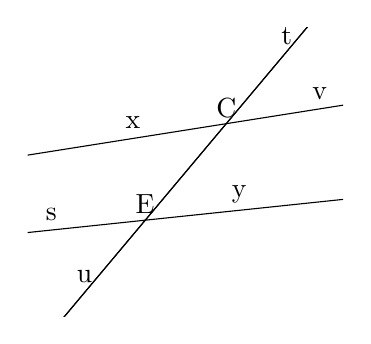
\begin{tikzpicture}[baseline,scale = 0.4]

    \tikzset{
      point/.style={
        thick,
        draw,
        cross out,
        inner sep=0pt,
        minimum width=5pt,
        minimum height=5pt,
      },
    }
    \clip (-5.019140905477899,-4.583099794098132) rectangle (4.998640241158492,4.58022221559489);
    	\draw[color={black}] (-48.098841810383796,-6.289634365773592)--(51.65768058972509,9.510246603289735);
	\draw[color={black}] (-30.853805264953884,-36.770133269710925)--(34.06774331338658,40.60035548530582);
	\draw[color={black}] (-51.011669987786746,-6.758512049620633)--(49.43504144440886,3.7988627404123747);
	\draw[color={black}] (-33.42495570370005,-39.83431104218686)--(31.49659287464043,37.536177712829925);
	\draw [color={black}] (4.25,2.5) node[anchor = center,scale=1, rotate = 0] {v};
	\draw [color={black}] (-1.68,1.56) node[anchor = center,scale=1, rotate = 0] {x};
	\draw [color={black}] (3.21,4.33) node[anchor = center,scale=1, rotate = 0] {t};
	\draw [color={black}] (1.7,-0.72) node[anchor = center,scale=1, rotate = 0] {y};
	\draw [color={black}] (-4.27,-1.35) node[anchor = center,scale=1, rotate = 0] {s};
	\draw [color={black}] (-3.21,-3.33) node[anchor = center,scale=1, rotate = 0] {u};
	\draw [color={black}] (1.29,2.03) node[anchor = center,scale=1, rotate = 0] {C};
	\draw [color={black}] (-1.29,-1.03) node[anchor = center,scale=1, rotate = 0] {E};

\end{tikzpicture}\\ \end{minipage}
	\item \begin{minipage}[t]{\linewidth} Quel est l'angle alterne-interne à l'angle $\widehat{DEu}$ ?\\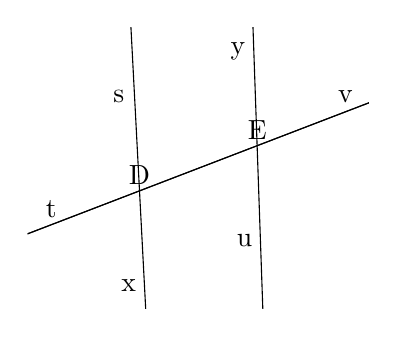
\begin{tikzpicture}[baseline,scale = 0.4]

    \tikzset{
      point/.style={
        thick,
        draw,
        cross out,
        inner sep=0pt,
        minimum width=5pt,
        minimum height=5pt,
      },
    }
    \clip (-5.417902132486009,-4.462624503354323) rectangle (5.417902132486009,4.464908380147888);
    	\draw[color={black}] (0.12218601786934635,50.68627725004538)--(3.647035184821962,-50.252196278883275);
	\draw[color={black}] (-44.81186047186567,-17.201661578174413)--(49.47976260435168,18.993501325900915);
	\draw[color={black}] (-4.483958665141602,49.21474083863809)--(0.8019729153957385,-51.646842171573866);
	\draw[color={black}] (-48.54618217785449,-18.635133376355615)--(45.74544089836289,17.560029527719713);
	\draw [color={black}] (1.47,-2.28) node[anchor = center,scale=1, rotate = 0] {u};
	\draw [color={black}] (1.26,3.71) node[anchor = center,scale=1, rotate = 0] {y};
	\draw [color={black}] (4.67,2.29) node[anchor = center,scale=1, rotate = 0] {v};
	\draw [color={black}] (-2.21,-3.71) node[anchor = center,scale=1, rotate = 0] {x};
	\draw [color={black}] (-2.52,2.28) node[anchor = center,scale=1, rotate = 0] {s};
	\draw [color={black}] (-4.67,-1.29) node[anchor = center,scale=1, rotate = 0] {t};
	\draw [color={black}] (1.87,1.22) node[anchor = center,scale=1, rotate = 0] {E};
	\draw [color={black}] (-1.87,-0.22) node[anchor = center,scale=1, rotate = 0] {D};

\end{tikzpicture}\\ \end{minipage}
\end{enumerate}
\end{multicols}

\end{exercice}


\end{document}
